\def\band{Grades 4--5}\def\packet{W94-U-v1}\documentclass[letterpaper,12pt]{article}
\usepackage[margin=0.65in,headheight=18pt,headsep=18pt,footskip=24pt]{geometry}
\usepackage{tikz,array,fancyhdr,amsmath}
\usepackage[T1]{fontenc}
\usepackage{lmodern}
\renewcommand{\familydefault}{\sfdefault}
\pagestyle{fancy}\fancyhf{}
\renewcommand{\headrulewidth}{0.35pt}\renewcommand{\footrulewidth}{0pt}
\fancyhead[L]{\small Week 94 / Calibration lab / \band}
\fancyfoot[L]{\footnotesize Bellingham Math Circle / Week 94 / \packet}
\fancyfoot[R]{\footnotesize\thepage}
\setlength{\parindent}{0pt}\setlength{\parskip}{9pt}
\pdfinfoomitdate=1\pdftrailerid{}\pdfsuppressptexinfo=15
\newcommand{\problem}[2]{\par\noindent\textbf{Problem #1:} #2\par}
\newcommand{\room}[1]{\vspace{#1}}
\newcommand{\ruler}[1]{\begin{tikzpicture}[x=12mm,y=10mm]\draw[line width=.8pt] (0,0)--(12,0);\foreach \i in {0,...,12}{\draw (\i,-.13)--(\i,.13);\pgfmathtruncatemacro{\lab}{\i+#1}\node[below,font=\small] at (\i,-.15){\lab};}\end{tikzpicture}}
\newcommand{\linepair}[3]{\begin{tikzpicture}[x=9.3mm,y=8mm]\node[anchor=east,font=\normalsize] at (-.4,0){#1};\draw (0,0)--(14,0);\foreach \i in {0,...,14}{\draw (\i,-.12)--(\i,.12);\node[below,font=\scriptsize] at (\i,-.15){\i};}\fill (#2,0) circle (2.3pt);\fill (#3,0) circle (2.3pt);\end{tikzpicture}}
\newcommand{\workbox}[1]{\begin{tikzpicture}\draw[gray!55] (0,0) rectangle (16.9,#1);\end{tikzpicture}}
\newcommand{\strips}{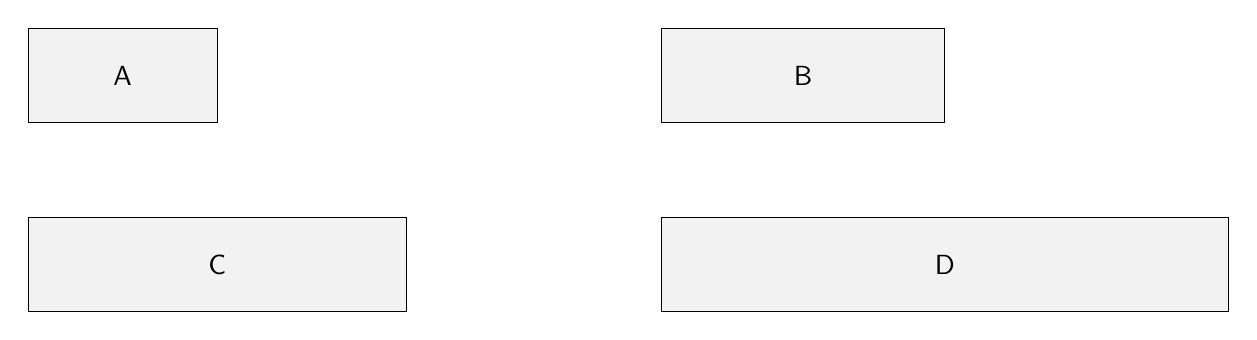
\begin{tikzpicture}[x=12mm,y=12mm]
\foreach \x/\y/\n/\s in {0/0/2/A,6.7/0/3/B,0/-2/4/C,6.7/-2/6/D}{\draw[fill=gray!10] (\x,\y) rectangle +(\n,1);\node at (\x+\n/2,\y+.5){\s};}
\end{tikzpicture}}
\newcommand{\unitrow}{\begin{tikzpicture}[x=12mm,y=12mm]\foreach\i in{0,...,11}{\draw(\i,0) rectangle +(1,1);}\end{tikzpicture}}
\newcommand{\addexample}{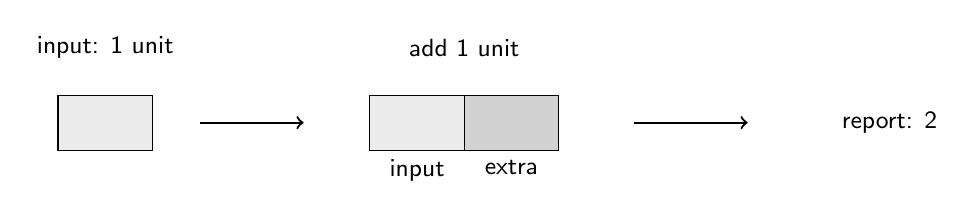
\begin{tikzpicture}[x=12mm,y=10mm,font=\small]
\node at (1.2,1.3){input: 1 unit};\draw[fill=gray!15] (.7,0) rectangle +(1,.7);
\draw[->,thick] (2.2,.35)--(3.3,.35);
\draw[fill=gray!15] (4,0) rectangle +(1,.7);\draw[fill=gray!35] (5,0) rectangle +(1,.7);
\node at (5,1.3){add 1 unit};\node[below] at (4.5,0){input};\node[below] at (5.5,0){extra};
\draw[->,thick] (6.8,.35)--(8,.35);\node at (9.5,.35){report: 2};
\end{tikzpicture}}
\newcommand{\affineexample}{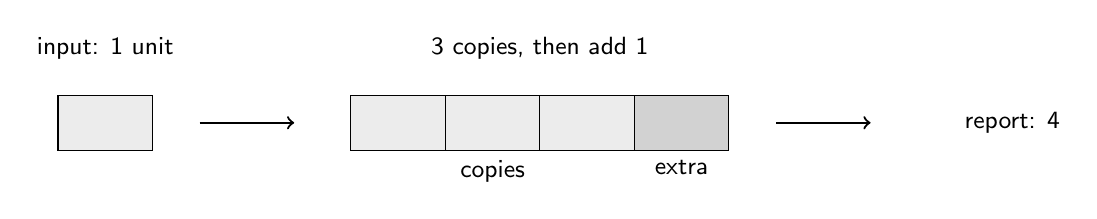
\begin{tikzpicture}[x=12mm,y=10mm,font=\small]
\node at (1,1.3){input: 1 unit};\draw[fill=gray!15] (.5,0) rectangle +(1,.7);
\draw[->,thick](2,.35)--(3,.35);
\foreach\i in{0,...,2}{\draw[fill=gray!15](3.6+\i,0)rectangle+(1,.7);}\draw[fill=gray!35](6.6,0)rectangle+(1,.7);
\node at (5.6,1.3){3 copies, then add 1};\node[below] at(5.1,0){copies};\node[below]at(7.1,0){extra};
\draw[->,thick](8.1,.35)--(9.1,.35);\node at(10.6,.35){report: 4};
\end{tikzpicture}}
\begin{document}\fontsize{12.5}{16.5}\selectfont
For Problems 1--2, a machine makes 1, 2, or 3 copies of the input length, then adds 0, 1, 2, 3, 4, 5, or 6 units. It keeps both choices fixed for the whole round. Each square in the paper row is one unit.
\begin{center}\affineexample\end{center}

\problem{1}{Play the machine. Secretly choose the number of copies and the extra amount. Your partner requests a strip's report. They may request more reports until they can name both choices. Reveal and switch jobs. How few requests can you manage?}

\begin{center}\begin{tabular}{|p{2.6cm}|p{4.7cm}|p{5.8cm}|}\hline
Round & Strips requested & Reports \\\hline
1\rule{0pt}{9mm}&&\\\hline 2\rule{0pt}{9mm}&&\\\hline 3\rule{0pt}{9mm}&&\\\hline 4\rule{0pt}{9mm}&&\\\hline
\end{tabular}\end{center}
\begin{center}\unitrow\end{center}
\begin{center}\strips\end{center}

\newpage

\problem{2}{A 2-unit strip reports 6. Find every possible machine. Choose a second strip that would separate all your possibilities, and show the reports you might get. Could a single first request ever identify a machine?}

\begin{center}\begin{tabular}{|p{3.8cm}|p{3.8cm}|p{5.5cm}|}\hline
Copies & Extra amount & Second strip and its report \\\hline
\rule{0pt}{17mm}&&\\\hline\rule{0pt}{17mm}&&\\\hline\rule{0pt}{17mm}&&\\\hline\rule{0pt}{17mm}&&\\\hline
\end{tabular}\end{center}
\vspace{5mm}\workbox{6.2}

\newpage

For the remaining problems, a stretch-and-shift machine multiplies every input length by the same positive number, then adds the same fixed amount. Fractions are allowed; the added amount may be negative.

\begin{center}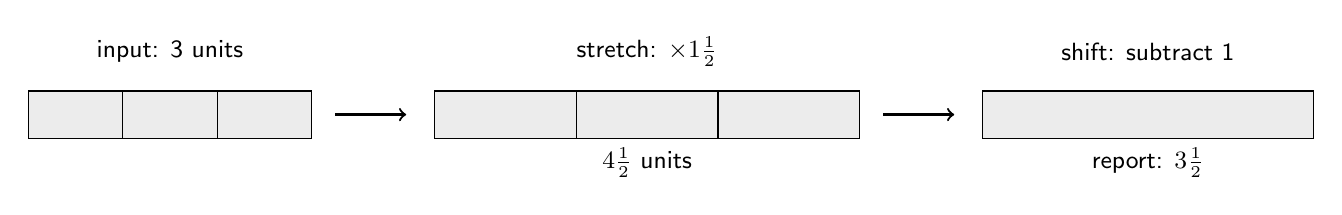
\begin{tikzpicture}[x=12mm,y=10mm,font=\small]
\node at(1.5,1.1){input: 3 units};
\foreach\i in{0,1,2}{\draw[fill=gray!15](\i,0)rectangle+(1,.6);}
\draw[->,thick](3.25,.3)--(4,.3);
\node at(6.55,1.1){stretch: $\times 1\frac12$};
\foreach\i in{0,1,2}{\draw[fill=gray!15](4.3+1.5*\i,0)rectangle+(1.5,.6);}
\node[below]at(6.55,0){$4\frac12$ units};
\draw[->,thick](9.05,.3)--(9.8,.3);
\node at(11.85,1.1){shift: subtract 1};
\draw[fill=gray!15](10.1,0)rectangle+(3.5,.6);
\node[below]at(11.85,0){report: $3\frac12$};
\end{tikzpicture}\end{center}

\problem{3}{Each machine gives these two reports. Find its rule and its reports for lengths 0, 4, and 10. Could a different stretch-and-shift rule give the same two known reports?}

\begin{center}\begin{tabular}{|p{6.2cm}|p{6.2cm}|}\hline
Machine A & Machine B \\\hline
2 units $\to$ 8 & 2 units $\to$ 8 \\
6 units $\to$ 16 & 6 units $\to$ 12 \\\hline
\rule{0pt}{15mm}Rule: & Rule:\\\hline
\rule{0pt}{12mm}0 units $\to$ & 0 units $\to$\\\hline
\rule{0pt}{12mm}4 units $\to$ & 4 units $\to$\\\hline
\rule{0pt}{12mm}10 units $\to$ & 10 units $\to$\\\hline
\end{tabular}\end{center}
\vspace{5mm}\workbox{3.5}

\newpage

\problem{4}{A machine claims to use one fixed stretch and shift. Could these three reports be correct? Find every way to repair the list by changing exactly one report.}

\begin{center}\begin{tabular}{|c|c|c|}\hline
2 units $\to$ 7 & 4 units $\to$ 11 & 6 units $\to$ 16 \\\hline
\end{tabular}\end{center}
\workbox{6.2}

\problem{5}{A machine gives 7, 11, and 15 for lengths 2, 4, and 6. Its rule stays fixed, but nobody promises stretch-and-shift. Make two complete report tables that fit these reports and disagree at length 8. Could any number of matching tests below length 8 force its report at 8?}

\begin{center}\begin{tabular}{|c|c|c|c|c|c|c|c|c|}\hline
Length & 1 & 2 & 3 & 4 & 5 & 6 & 7 & 8\\\hline
Table A\rule{0pt}{15mm}&\hspace{7mm}&7&\hspace{7mm}&11&\hspace{7mm}&15&\hspace{7mm}&\hspace{7mm}\\\hline
Table B\rule{0pt}{15mm}&&7&&11&&15&&\\\hline
\end{tabular}\end{center}
\room{2cm}

\newpage

For Problems 6--7, the machine uses one fixed stretch and shift. The reference lengths are exact. Each displayed report may be up to 1 above or below its true report.
\begin{center}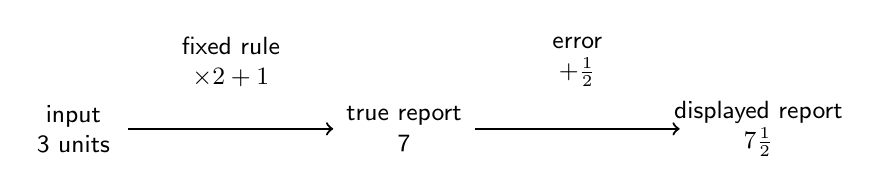
\begin{tikzpicture}[font=\small]
\node[align=center] at(0,0){input\\3 units};
\draw[->,thick] (.7,0)--(3.3,0);\node[align=center] at(2,.85){fixed rule\\$\times2+1$};
\node[align=center] at(4.2,0){true report\\7};
\draw[->,thick] (5.1,0)--(7.7,0);\node[align=center] at(6.4,.85){error\\$+\frac12$};
\node[align=center] at(8.7,0){displayed report\\$7\frac12$};
\end{tikzpicture}\end{center}

\problem{6}{For each pair of reference strips, find the smallest and largest possible stretch. Give a machine that reaches each extreme.}

\begin{center}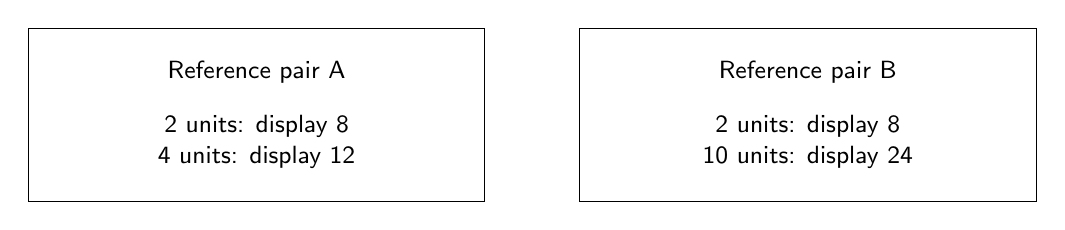
\begin{tikzpicture}[font=\small]
\node[draw,minimum width=5.8cm,minimum height=2.2cm,align=center] at(0,0){Reference pair A\\[3mm]2 units: display 8\\4 units: display 12};
\node[draw,minimum width=5.8cm,minimum height=2.2cm,align=center] at(7,0){Reference pair B\\[3mm]2 units: display 8\\10 units: display 24};
\end{tikzpicture}\end{center}
\vspace{3mm}\workbox{4.5}

\problem{7}{Choose two exact reference lengths from 1 to 10 units before seeing any reports. Which pair gives the smallest guaranteed bound on how wide the range of possible stretches can be, even with the least helpful allowed errors? Could repeating one reference ten times guarantee the same result?}

\vspace{3mm}\workbox{4.5}
\end{document}
